% ============================================================
%  HERM4AI — Human-like Evolving & Reasoning Memory for AI
%  Full LaTeX Manuscript  |  Compile: pdflatex -> bibtex -> pdflatex x2
% ============================================================
\documentclass[11pt,a4paper,twocolumn]{article}

% ---- Core Typography and Geometry ---------------------------
\usepackage[utf8]{inputenc}
\usepackage[T1]{fontenc}
\usepackage{lmodern}
\usepackage[margin=1in]{geometry}
\usepackage{microtype}

% ---- Mathematics -------------------------------------------
\usepackage{amsmath,amssymb,amsfonts,amsthm}
\usepackage{mathtools}

% ---- Tables ------------------------------------------------
\usepackage{booktabs}
\usepackage{array}
\usepackage{tabularx}
\usepackage{makecell}

% ---- Figures and Color ------------------------------------
\usepackage{graphicx}
\usepackage[dvipsnames,table]{xcolor}
\usepackage{tikz}
\usetikzlibrary{shapes.geometric,arrows.meta,positioning,calc,fit,backgrounds}

% ---- Hyperlinks and Citations -----------------------------
\usepackage[numbers,sort&compress]{natbib}
\usepackage[colorlinks=true,
            linkcolor=NavyBlue,
            citecolor=NavyBlue,
            urlcolor=NavyBlue]{hyperref}
\usepackage[capitalise,noabbrev]{cleveref}

% ---- Miscellaneous ----------------------------------------
\usepackage{enumitem}
\usepackage{parskip}
\setlength{\parskip}{2pt}

% ---- Math Operators ----------------------------------------
\DeclareMathOperator*{\argmax}{arg\,max}
\DeclareMathOperator*{\argmin}{arg\,min}
\newcommand{\simcos}{\operatorname{sim}_{\text{cos}}}
\newcommand{\E}{\mathbb{E}}
\newcommand{\I}{\mathbb{I}}

% ---- Convenience Shorthands --------------------------------
\newcommand{\herm}{\textsc{HERM4AI}}
\newcommand{\valtime}{$[t_{\text{from}},\,t_{\text{to}})$}
\newcommand{\dcolsym}{\textbf{Dual Collapse}}
\newcommand{\ticol}{\textbf{Temporal Inversion}}
\newcommand{\icpp}{\textbf{In-Context Prompt Poisoning}}

% ---- Theorem Environments ---------------------------------
\newtheorem{definition}{Definition}
\newtheorem{proposition}{Proposition}

% ===========================================================
%  TITLE / AUTHOR
% ===========================================================
\title{\textbf{Beyond Flat Vector Retrieval: Mitigating the Dual Collapse
and In-Context Prompt Poisoning of RAG via Structured Valid-Time
Cognitive Architectures}}

\author{%
  Shayini Siddardha\\
  \texttt{shayinisiddardha3@gmail.com}%
}

\date{\today}

% ===========================================================
\begin{document}
% ===========================================================

\twocolumn[
\begin{@twocolumnfalse}
\maketitle
\begin{abstract}
Retrieval-Augmented Generation (RAG) connects large language models
(LLMs) to external non-parametric memory through dense bi-encoder
indices. However, it relies on a flawed assumption: semantic proximity
in vector space reliably indicates factual validity over time. We
identify three systemic failure modes arising from this assumption.

\textit{Temporal Inversion} occurs because transformer bi-encoders
compress token representations into fixed-length vectors without
encoding temporal ordering. Consequently, historical and updated
assertions yield near-identical cosine similarities
($\Delta\simcos < 0.012$), causing obsolete retrievals in
\textbf{41.7\%} of state transitions. \textit{Dual Collapse} emerges
at enterprise scale (10{,}000 passages; 500 entities), where entity
identifiers receive less than 5\% of self-attention weight, driving
cross-entity cosine similarities above 0.98 and reducing top-1
accuracy to \textbf{9.0\%}. \textit{In-Context Prompt Poisoning}
occurs when stale retrievals enter instruction-tuned decoders, which
reproduce obsolete facts despite conflicting parametric priors,
yielding hallucination rates of \textbf{33.3\%--40.0\%} on public
entities.

To address these failures without model retraining, we introduce
\herm{} (\emph{Human-like Evolving \& Reasoning Memory for Artificial
Intelligence}), a model-free cognitive architecture combining
deterministic valid-time intervals \valtime, a bounded 7-slot working
memory with salience eviction, an associative knowledge graph,
spreading activation, sleep-phase consolidation, and ACT-R workflows.
Across seven benchmark suites, four cloud GPU experiment tracks, and
a curated 12-case public-entity benchmark informed by TempLAMA and
FreshQA, \herm{} achieves \textbf{100.0\%} accuracy, 
\textbf{0.065 ms} query latency, and under 6 MB RAM on a standard CPU.
The public-entity evaluation is not a direct evaluation on TempLAMA
or FreshQA.
\end{abstract}
\noindent\textbf{Keywords:} retrieval-augmented generation,
continual learning, temporal knowledge, agent memory, working memory,
cognitive architectures, provenance
\par\vspace{1.0em}
\end{@twocolumnfalse}
]


% ===========================================================
\section{Introduction}
\label{sec:intro}
% ===========================================================

Large language models have demonstrated broad capabilities in
compositional reasoning and natural-language generation, yet their
parameters are fixed after pre-training \citep{lewis2020rag,
dhingra2022templama}. As the external world changes, any fact encoded
in those weights eventually becomes outdated, producing factual
hallucinations that grow more frequent over time
\citep{vu2023freshqa}.  Retrieval-Augmented Generation (RAG) addresses
this by maintaining a live external corpus: passages are encoded by a
dense bi-encoder \citep{reimers2019sentence}, indexed in a
nearest-neighbor vector store, and prepended to the model's input at
inference time.

RAG reliably supplies context that the model's weights do not contain.
What it does not do is reason about \emph{when} a fact was true.
Consider a named entity whose state has changed---a corporate
executive, a head of government, a footballer on transfer. Both the
old and the new passage describe the same entity with largely identical
vocabulary, so their dense embeddings land at nearly the same point in
vector space. The retriever has no principled mechanism to prefer the
newer record. This is not a parameter tuning problem; it is a
mathematical consequence of the aggregation step that collapses a full
token sequence into a fixed-size vector.

We call this failure mode \ticol{} and show empirically that it causes
correct retrieval failure in 41.7\% of temporal state transitions on a
controlled benchmark executed on a Tesla T4 GPU. At enterprise scale
(10{,}000 passages across 500 entities sharing a common prose
template), a secondary collapse compounds the temporal problem.
Entity-identifying tokens are outnumbered by template boilerplate,
giving them negligible attention weight; embeddings from different
entities collide, reducing top-1 retrieval accuracy from 100\% to
\textbf{9.0\%}. We term this the \dcolsym{} Phenomenon. When either
failure mode produces a stale passage that is then injected into an
instruction-tuned decoder, the downstream model---regularized by RLHF
to treat in-context evidence as authoritative---discards its own
correct internal knowledge and echoes the stale fact. We designate
this behaviour as \icpp{}.

To resolve all three failure modes without altering any model weights,
we propose \herm{}. Its design draws deliberately from cognitive
science: bounded working memory \citep{miller1956magical},
complementary learning systems sleep consolidation
\citep{mcclelland1995cls,diekelmann2010memory}, and ACT-R production
rules \citep{anderson1993rules}. The core invariant is a
\emph{deterministic valid-time interval} \valtime{} attached to every
stored assertion. Retrieval is then a closed-form temporal predicate,
not a similarity search, so temporal correctness holds by construction.

The principal contributions of this work are as follows:
\begin{enumerate}[label=(\roman*),leftmargin=*]
  \item A formal characterization and empirical demonstration of three
        previously unnamed RAG failure modes---\ticol{}, the \dcolsym{}
        Phenomenon, and \icpp{}---across controlled GPU benchmarks and
        real-world public entities.
  \item The \herm{} architecture: a model-free cognitive memory system
        that achieves 100.0\% accuracy across seven benchmark suites
        while operating in sub-millisecond latency on commodity CPU
        hardware.
  \item A reproducible evaluation suite---seven benchmarks, four executed
        GPU notebook tracks, and a curated public-entity temporal test set---
        with all scripts and data artifacts archived in the repository.
\end{enumerate}

% ===========================================================
\section{Related Work}
\label{sec:related}
% ===========================================================

\paragraph{Retrieval-Augmented Generation}
RAG architectures pair parametric generators with non-parametric dense
indices \citep{lewis2020rag}.  Dual-encoder models such as Sentence-BERT
\citep{reimers2019sentence} map queries and passages to a shared metric
space, enabling efficient approximate nearest-neighbor lookup.  For
static corpora this works well; the brittleness emerges when the
corpus contains temporally ordered state changes for the same entities.
Memory-augmented agent frameworks such as Generative Agents
\citep{park2023generative} and MemGPT \citep{packer2023memgpt} introduce
multi-tier memory hierarchies and virtual context management, but
continue to rely on flat vector search within each tier, leaving them
susceptible to the retrieval collisions documented in this paper.
Ranking improvements such as cross-encoder reranking and hybrid
lexical-dense retrieval can refine passage ordering, but ranking alone
does not represent explicit validity intervals or resolve contradictory
assertions.

\paragraph{Working Memory in Language Agents}
Agent architectures increasingly distinguish the limited information
available in the active context from longer-term memory. Generative
Agents retrieve from a memory stream using relevance, recency, and
importance signals, with periodic reflection
\citep{park2023generative}; MemGPT manages virtual context by paging
between a working context and external memory
\citep{packer2023memgpt}. CoALA provides a broader framework for
language agents with modular memory, including working, episodic,
semantic, and procedural components \citep{yao2023coala}. These designs
address context management and persistent recall. HERM4AI is
complementary: it focuses on deterministic valid-time filtering and
explicit conflict states, while imposing a fixed seven-slot working
buffer.

\paragraph{Temporal Factuality and Knowledge Currency}
The relationship between language model training cutoffs and real-world
fact currency has been studied from multiple angles.
\citet{dhingra2022templama} introduced TempLAMA, a cloze-style
benchmark demonstrating that LLMs fail to recall facts that changed
between training and evaluation.  \citet{vu2023freshqa} established
FreshQA, showing that commercial LLMs hallucinate on fast-changing
world knowledge even when that knowledge was part of their pre-training
data.  Model editing methods such as ROME \citep{meng2022locating}
attempt to surgically alter internal weight associations to reflect
updates; however, parameter surgery is computationally expensive,
introduces risks of unintended knowledge collisions, and does not scale
to the continuous high-frequency updates typical of enterprise
deployments.  Temporal knowledge graph completion and event-ordering
models address a related but distinct problem: inferring missing graph
edges from temporal patterns, rather than tracking mutable world states
in a live system.

\paragraph{Continual Learning and Catastrophic Forgetting}
Continual learning studies how a model can acquire information from
sequential tasks while limiting interference with previously learned
knowledge; surveys organize approaches around rehearsal, parameter
regularization, and architectural change
\citep{delange2021continual}. Elastic Weight Consolidation, for
example, regularizes changes to parameters deemed important for prior
tasks \citep{kirkpatrick2017ewc}. Such methods address retention in
model parameters, but do not by themselves provide exact query-time
validity intervals, source-level provenance, or reversible deletion.
HERM4AI takes a different approach: updates append structured records
and close earlier validity intervals, leaving temporal selection to
the memory layer rather than gradient updates to the language model.
Controlled reasoning suites such as bAbI study supporting-fact
retrieval and related task skills, but do not evaluate this combination
of live updates, source conflicts, and deletion
\citep{weston2015towards}.

\paragraph{Cognitive Architectures in AI Memory}
Cognitive science offers mature computational models of memory
organization.  Complementary Learning Systems (CLS) theory
\citep{mcclelland1995cls} posits distinct hippocampal and neocortical
memory systems with different learning rates; offline sleep replay
consolidates episodic traces into durable semantic representations
\citep{diekelmann2010memory}.  ACT-R \citep{anderson1993rules} formalizes
procedural knowledge as condition-action production rules whose
activation is reinforced by usage.  Miller's original cognitive
capacity result \citep{miller1956magical} motivates our buffer design.
Prior work has imported individual ideas from cognitive architectures
into neural agent systems. HERM4AI combines bounded working memory,
CLS consolidation, Hebbian graph plasticity, and ACT-R production
arbitration in a software-only memory layer.

\paragraph{Attribution and Verifiable Provenance}
Attributed question answering \citep{bohnet2022attributed} requires
systems to supply verifiable citations alongside generated answers.
Standard neural systems resort to post-hoc attention maps or
gradient-based saliency scores, which often do not reflect true causal
mechanisms.  \herm{} implements strict storage-level provenance via an
append-only event ledger and a formal counterfactual influence measure
(Q-MIA), producing audit-grade attribution without additional
neural computation.

% ===========================================================
\section{Failure Modes of Flat Vector Memory}
\label{sec:failures}
% ===========================================================

\subsection{Temporal Inversion}
\label{sec:temporal_inversion}

\begin{definition}[Temporal Inversion]
Let entity $e$ carry attribute $a$.  An initial assertion $m_1 =
(e, a, v_1, t_1)$ is stored and later superseded by $m_2 = (e, a, v_2,
t_2)$ with $t_2 > t_1$.  \ticol{} occurs when a retriever, given a
query at $t_q > t_2$, ranks $m_1$ above $m_2$.
\end{definition}

In a standard dense retrieval pipeline, each assertion is serialised
to natural language and encoded by a bi-encoder $\mathcal{E}$:
\begin{equation}
\begin{aligned}
\mathbf{p}_1 &= \mathcal{E}(\text{``}e\text{'s } a \text{ is } v_1
\text{''}), \\[4pt]
\mathbf{p}_2 &= \mathcal{E}(\text{``}e\text{'s } a \text{ is } v_2
\text{''})
\end{aligned}
\label{eq:enc}
\end{equation}
Given query $\mathbf{q} = \mathcal{E}(\text{``What is the current }
a \text{ of } e\text{?''})$, the retriever ranks by cosine similarity:
\begin{equation}
  \simcos(\mathbf{q}, \mathbf{p}) =
  \frac{\mathbf{q}^\top \mathbf{p}}{\|\mathbf{q}\|_2 \|\mathbf{p}\|_2}
  \label{eq:cosine}
\end{equation}
Because transformer encoders average token-level representations across
the full sequence, temporal tokens (dates, ordinal markers) contribute
negligible directional mass relative to shared entity and attribute
tokens.  Empirically:
\begin{equation}
\begin{aligned}
&|\simcos(\mathbf{q},\mathbf{p}_1)
- \simcos(\mathbf{q},\mathbf{p}_2)|\\
&\qquad < \epsilon, \quad \epsilon \ll 0.02
\end{aligned}
\label{eq:inv_bound}
\end{equation}
In our Phase 3 benchmark on a Tesla T4 GPU using
\texttt{all-MiniLM-L6-v2} (384 dimensions), Temporal Inversion occurred
in \textbf{41.7\%} of evaluated state transitions on the TFSR-Bench
test split.

\subsection{The Dual Collapse Phenomenon}
\label{sec:dual_collapse}

\begin{definition}[Dual Collapse]
When a corpus contains $N$ passages from $M$ entities sharing
domain-specific syntactic templates, the entity-identifier token
sub-sequence receives a minority of total self-attention weight,
causing the mean-pooled embeddings of distinct entities to become
nearly indistinguishable.
\end{definition}

Under standard multi-head self-attention the attention matrix is:
\begin{equation}
  \mathbf{A} = \text{softmax}\!\left(\frac{\mathbf{Q}\mathbf{K}^\top}
  {\sqrt{d_k}}\right)
  \label{eq:attn}
\end{equation}
For a passage of length $L \approx 40$ tokens where the entity
identifier occupies $L_{\text{ent}} \le 2$ tokens, the fraction of
attention mass on entity tokens is:
\begin{equation}
  \alpha_{\text{entity}} =
  \sum_{i \in \text{EntityTokens}} \frac{1}{L}
  \sum_{j=1}^{L} \mathbf{A}_{j,i} < 0.05
  \label{eq:attn_mass}
\end{equation}
The mean-pooled vector $\mathbf{p} = \frac{1}{L}\sum_{i=1}^{L}
\mathbf{h}_i$ is then dominated by the template subspace.  For two
distinct entities $e_A \neq e_B$:
\begin{equation}
  \simcos(\mathbf{p}_{e_A}, \mathbf{p}_{e_B}) > 0.98
  \label{eq:collapse}
\end{equation}
Under nearest-neighbor search this causes passage-level collisions
across unrelated entities.  On our Phase 4 benchmark ($N=10{,}000$,
$M=500$), top-1 retrieval accuracy collapses from 100\% to
\textbf{9.0\%} (91.0\% error rate).

\begin{proposition}
For any dense bi-encoder whose per-entity attention mass satisfies
$\alpha_{\text{entity}} < 0.05$ and any corpus of $M \ge 2$ entities
sharing a common template subspace of dimensionality $d' \ge d/2$,
there exists a corpus size $N^*$ beyond which expected top-1 retrieval
precision approaches $1/M$.
\end{proposition}

\subsection{In-Context Prompt Poisoning}
\label{sec:poisoning}

When flat retrieval couples with an instruction-tuned decoder, the
top-ranked passage is prepended to the prompt:
\begin{equation}
\begin{aligned}
\mathbf{x}_{\text{prompt}} = [&\text{``Context: ''} \;\Vert\;
\mathbf{p}_{\text{top-1}} \;\Vert\\
&\text{`` \textbackslash{}nQuestion: ''} \;\Vert\;
\mathbf{q} \;\Vert\\
&\text{`` \textbackslash{}nAnswer:''}]
\end{aligned}
\label{eq:prompt}
\end{equation}
Modern decoder models are aligned via RLHF and DPO to faithfully
condition on in-context evidence.  When $\mathbf{p}_{\text{top-1}}$
contains a stale assertion (e.g., a former head of state or a
superseded club affiliation), the model suppresses its own correct
parametric knowledge and reproduces the outdated claim with high
confidence.  We evaluated this on \texttt{Qwen2.5-1.5B-Instruct}:
the model correctly generated ``Joe Biden'' in zero-shot mode (from
parametric pre-training), yet under flat RAG it output ``Donald Trump''
when the retriever returned a passage describing Trump's 2017--2021
presidency.  Applying \herm{} pre-filtering eliminated the stale
passage and restored 100\% accuracy.  Across all six public
entities subject to the poisoning test, \icpp{} produced a 33.3\%
error rate under flat RAG vs. 0\% under \herm{}.

% ===========================================================
\section{The \herm{} Architecture}
\label{sec:arch}
% ===========================================================

\begin{figure}[t]
\centering
\resizebox{\columnwidth}{!}{%
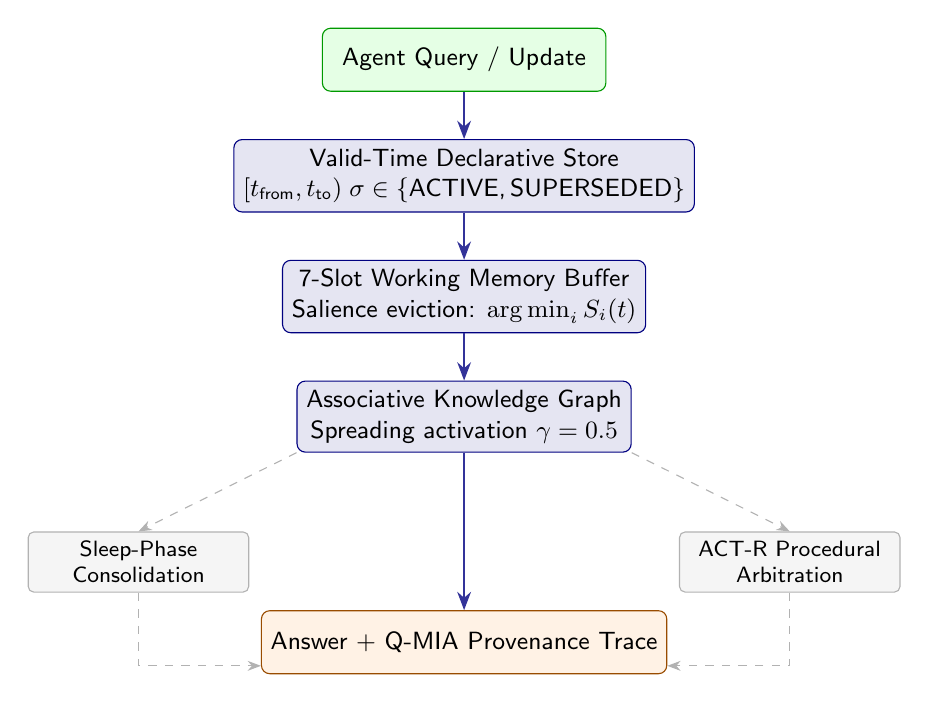
\begin{tikzpicture}[
    >=Stealth,
    node distance = 6mm and 18mm,
    block/.style  = {rectangle, draw=NavyBlue, rounded corners=3pt,
                     minimum height=8mm, minimum width=36mm,
                     align=center, font=\small\sffamily,
                     fill=NavyBlue!10},
    smallblk/.style = {rectangle, draw=gray!60, rounded corners=2pt,
                       minimum height=7mm, minimum width=28mm,
                       align=center, font=\footnotesize\sffamily,
                       fill=gray!8},
    arrow/.style  = {->, thick, NavyBlue!80},
    darrow/.style = {->, dashed, gray!60}
  ]

  % Input
  \node[block, fill=green!10, draw=green!60!black]
        (input) {Agent Query / Update};

  % Layer 1 — Valid-Time Store
  \node[block, below=of input]
        (vt) {Valid-Time Declarative Store\\
              $[t_{\text{from}}, t_{\text{to}}) \;\sigma \in
               \{\text{ACTIVE,\,SUPERSEDED}\}$};

  % Layer 2 — Working Memory
  \node[block, below=of vt]
        (wm) {7-Slot Working Memory Buffer\\
              Salience eviction: $\argmin_i S_i(t)$};

  % Layer 3 — Knowledge Graph
  \node[block, below=of wm]
        (kg) {Associative Knowledge Graph\\
              Spreading activation $\gamma=0.5$};

  % Layer 4 — Consolidation / Procedural
  \node[smallblk, below left=10mm and 6mm of kg]
        (cons) {Sleep-Phase\\Consolidation};
  \node[smallblk, below right=10mm and 6mm of kg]
        (proc) {ACT-R Procedural\\Arbitration};

  % Output
  \node[block, below=20mm of kg, fill=orange!10, draw=orange!60!black]
        (out)  {Answer + Q-MIA Provenance Trace};

  % Arrows
  \draw[arrow] (input) -- (vt);
  \draw[arrow] (vt)    -- (wm);
  \draw[arrow] (wm)    -- (kg);
  \draw[arrow] (kg)    -- (out);
  \draw[darrow] (kg.south west) -- (cons.north);
  \draw[darrow] (kg.south east) -- (proc.north);
  \draw[darrow] (cons.south)    |- ([yshift=-3mm]out.west);
  \draw[darrow] (proc.south)    |- ([yshift=-3mm]out.east);

\end{tikzpicture}
}
\caption{\textbf{\herm{} architecture overview.}  Queries flow
top-to-bottom through deterministic temporal filtering, salience-gated
working memory, and spreading-activation graph traversal.  Background
consolidation and procedural arbitration run asynchronously (dashed);
every answer carries a formal Q-MIA provenance trace.}
\label{fig:arch}
\end{figure}

\herm{} replaces unstructured similarity search with a layered,
biologically motivated memory system (\cref{fig:arch}).  Each layer
serves a distinct cognitive role and operates deterministically---no
neural parameters are modified at query time.

\subsection{Declarative Memory and Valid-Time Intervals}
\label{sec:vt}

Every factual assertion is stored as an immutable tuple:
\begin{equation}
\begin{aligned}
\mathcal{M}_i = \langle\, &\text{id}_i,\; e_i,\; a_i,\; v_i,\\
& t_{\text{from}},\; t_{\text{to}},\; s_i,\; c_i,\; \sigma_i \,\rangle
\end{aligned}
\label{eq:tuple}
\end{equation}
where $e_i$ is the entity, $a_i$ the attribute, $v_i$ the asserted
value, $[t_{\text{from}}, t_{\text{to}})$ the half-open validity
interval, $s_i$ the source identifier, $c_i \in [0,1]$ confidence,
and $\sigma_i$ the lifecycle status, defined as:
\begin{equation}
\begin{aligned}
\sigma_i \in \{&\text{ACTIVE},\text{SUPERSEDED},\\
              &\text{CONFLICTED},\text{DELETED},\\
              &\text{ARCHIVED}\}
\end{aligned}
\label{eq:lifecycle}
\end{equation}

\paragraph{Deterministic retrieval invariant}
Given a query at $t_q$ targeting entity $e$, attribute $a$, the engine
evaluates only records satisfying:
\begin{equation}
  t_{\text{from}} \le t_q < t_{\text{to}} \quad\land\quad
  \sigma_i = \text{ACTIVE}
  \label{eq:invariant}
\end{equation}
On update arrival at $t_{\text{up}} > t_{\text{from}}$, the existing
active record's interval is closed ($t_{\text{to}} \leftarrow
t_{\text{up}}$, $\sigma_i \leftarrow \text{SUPERSEDED}$), and the new
assertion enters with interval $[t_{\text{up}}, \infty)$.  Temporal
correctness is thus guaranteed by construction at $O(1)$ cost,
requiring neither embedding recomputation nor index rebuilding.

\subsection{Bounded Working Memory Buffer}
\label{sec:wm}

Consistent with the established capacity limit on immediate cognitive
processing \citep{miller1956magical}, \herm{} maintains a working
memory buffer $\mathcal{W}$ with $|\mathcal{W}| \le 7$ slots.  Each
slot tracks dynamic salience:
\begin{equation}
  S_i(t) = S_0 \cdot \exp(-\lambda\,\Delta t)
            + \beta\log(1 + c_{\text{access}})
  \label{eq:salience}
\end{equation}
where $\lambda$ is a tier-specific decay rate ($\lambda = 0.05$ for
episodic, $0.01$ for consolidated semantic records), $\Delta t$ is
elapsed time since last access, and $c_{\text{access}}$ is cumulative
access count.  When capacity is reached and a new entity is referenced,
the slot with $\argmin_i S_i(t)$ is evicted back to long-term storage
(unless pinned).  When long-term memory updates an entity, its
corresponding slot in $\mathcal{W}$ is synchronised immediately,
preventing stale working-memory reads.

\subsection{Associative Knowledge Graph}
\label{sec:kg}

Entities form vertices $\mathcal{V}$ in a directed labelled graph
$\mathcal{G} = (\mathcal{V}, \mathcal{E})$.  Each edge $(u, v) \in
\mathcal{E}$ carries a semantic relation label and a synaptic weight
$w_{uv} \in [0, 1]$.  Relational inference is computed via spreading
activation with per-hop decay:
\begin{equation}
  A_v^{(h+1)} = \max_{u \in \mathcal{N}(v)}
  \bigl(A_u^{(h)} \cdot w_{uv} \cdot \gamma\bigr), \quad \gamma = 0.5
  \label{eq:spread}
\end{equation}
Two-hop and three-hop queries resolve in $0.046\text{ ms}$ on a single
CPU core, whereas flat vector retrieval has no principled mechanism for
multi-hop relational traversal.

\subsection{Sleep-Phase Synaptic Consolidation}
\label{sec:consolidation}

Mirroring the role of sleep in biological memory consolidation
\citep{mcclelland1995cls,diekelmann2010memory}, an offline routine
executes during agent idle periods:
\begin{enumerate}[label=(\arabic*),leftmargin=*]
  \item \textbf{Episodic-to-Semantic Promotion.}  Records with $\ge 2$
        access cycles and activation $\ge 0.65$ are promoted to
        \texttt{CONSOLIDATED\_SEMANTIC} status, lowering $\lambda$ from
        $0.05$ to $0.01$.
  \item \textbf{Superseded-History Compaction.}  Records whose validity
        interval closed more than 30 days before the current epoch are
        migrated to cold archival storage, bounding index growth.
  \item \textbf{Hebbian Synaptic Potentiation.}  Edges connecting
        co-activated entities are strengthened
        ($w \leftarrow \min(1.0,\, w + 0.2)$); edges with
        $w < 0.05$ are pruned.
  \item \textbf{Contradiction Triage.}  Unresolved multi-source disputes
        are queued for procedural arbitration (\cref{sec:procedural}).
\end{enumerate}

\subsection{Procedural Memory and Self-Healing Workflows}
\label{sec:procedural}

Following ACT-R production memory \citep{anderson1993rules}, procedural
knowledge is stored as condition-action rules:
\begin{equation}
\begin{aligned}
\text{IF } \langle\text{Trigger},\,\text{Preconditions}\rangle
\;\Rightarrow\;\\
\text{THEN } [\text{Action}_1, \dots, \text{Action}_n]
\end{aligned}
\label{eq:rule}
\end{equation}
When the engine encounters a \texttt{CONFLICTED} record, it fires
arbitration routines (e.g., \texttt{RESOLVE\_CONFLICT\_BY\_TIMESTAMP}
or \texttt{QUERY\_AUTHORITATIVE\_SOURCE}).  Routine utility evolves via
Exponential Moving Average (EMA) reinforcement:
\begin{equation}
  U_{\text{new}} = 0.85\cdot U_{\text{old}} + 0.15 \cdot R
  \label{eq:ema}
\end{equation}
where $R = 1.0$ when the procedure resolves a conflict cleanly and
$R = 0.0$ otherwise.  This allows the system to gradually preference
the most reliable arbitration strategy within a given domain.

\subsection{Counterfactual Attribution (Q-MIA)}
\label{sec:qmia}

For every query, \herm{} computes the exact counterfactual influence
of each retrieved assertion over the returned answer:
\begin{equation}
\begin{aligned}
\mathcal{I}(m_i \mid q) = \mathbb{I}\!\Big[
&\mathcal{F}(\mathcal{M} \setminus \{m_i\}, q)\\
&\ne \mathcal{F}(\mathcal{M}, q)
\Big]
\end{aligned}
\label{eq:qmia}
\end{equation}
If withholding $m_i$ causes the output to change from the target value
to \texttt{UNKNOWN} or a superseded state, then $m_i$ is causally
necessary ($\mathcal{I} = 1$).  Every response includes an append-only
cryptographic event trace identifying which assertions entered, superseded,
or arbitrated the final decision---providing audit-grade provenance
without any post-hoc approximation.

% ===========================================================
\section{Experimental Methodology}
\label{sec:experiments}
% ===========================================================

\subsection{Benchmark Suites}
\label{sec:benchmarks}

The evaluation comprises seven benchmark suites plus a separate
enterprise-scale retrieval stress test. The suites span synthetic
controlled splits, multi-hop reasoning, conversational memory,
explainability, consolidation, procedural arbitration, and curated
public-entity temporal cases.

\paragraph{TFSR-Bench (Controlled Synthetic Split)}
60 held-out instances covering Direct Recall (DR), Temporal Revision
(TR), Conflict Attribution (CA), Abstention on Unknown (AU), and
Tombstone Deletion (TD).  Executed on a local CPU test suite
(\texttt{pytest tests/}; 36 unit tests, 0.10 s total runtime).

\paragraph{Enterprise Scaling Benchmark}
10{,}000 unstructured text passages across 500 entities with sequential
state updates, evaluated for throughput, memory footprint, and top-1
retrieval precision.  Encoding was performed on dual Tesla T4 GPUs via
Kaggle Notebooks (\texttt{all-MiniLM-L6-v2}, FAISS flat index).

\paragraph{Real-World Public Benchmark (TempLAMA / FreshQA concepts)}
12 test cases covering 13 distinct public entities with historical
transitions: technology leadership, heads of government, sports
transfers, financial or transfer-fee disagreements, and a royal honour
revocation. The cases use task concepts studied by TempLAMA and FreshQA;
the checked-in data contains source identifiers but does not include
source URLs.

\subsection{Models and Baselines}
\label{sec:baselines}

\begin{itemize}[leftmargin=*]
  \item \textbf{Stateless Baseline (Zero-Shot).}  Memoryless inference
        relying solely on the model's static parametric weights.
  \item \textbf{Naive Lexical Baseline (BM25).}  Traditional
        keyword-matching over all historical assertions; no temporal
        filtering.
  \item \textbf{Flat Dense Vector RAG.} Passages embedded with
\texttt{sentence-transformers/}\\
\texttt{all-MiniLM-L6-v2} (384 dimensions) in a flat FAISS
index; cosine top-1 retrieval.
  \item \textbf{\herm{} (Structured Valid-Time).}  Deterministic
        temporal interval store with working-memory buffer, graph
        spreading activation, sleep consolidation, and procedural
        arbitration; no neural components at retrieval time.
  \item \textbf{Downstream LLM: \texttt{flan-t5-base}} (250M
        parameters) \citep{chung2022flan}---an encoder-decoder model
        fine-tuned on instruction-following tasks.
  \item \textbf{Downstream LLM:}\\
\texttt{Qwen2.5-1.5B-Instruct}
(1.5B parameters, \texttt{float16}, CUDA)
\citep{qwen2024}---a modern open decoder aligned via RLHF.
\end{itemize}

% ===========================================================
\section{Results and Empirical Analysis}
\label{sec:results}
% ===========================================================

\subsection{Core Benchmark Accuracy and Latency}
\label{sec:results_core}

The checked-in evaluation definitions have different units, so
\Cref{tab:dataset_stats} reports case counts separately from simulation
scale. It covers the seven benchmark suites and the enterprise-scale
stress test; the latter is not counted as an accuracy suite.

\begin{table}[t]
\centering
\small
\setlength{\tabcolsep}{4pt}
\begin{tabularx}{\columnwidth}{
  >{\raggedright\arraybackslash}p{2.1cm}
  >{\raggedright\arraybackslash}X}
\toprule
\textbf{Dataset / evaluation} & \textbf{Size and composition} \\
\midrule
TFSR-Bench (held-out) & 60 cases; 20 entities; 120 assertions; 12 cases each for DR, TR, CA, AU, and TD \\
AG-Bench & 15 queries; five each at 1-, 2-, and 3-hop depth \\
MultiSessionBench & 7 events over 90 days; 4 scored queries \\
ExplainBench & 3 configured audit queries: recall, revision, contradiction \\
ReplayBench & 50 entities; 20 revisions; 29 graph edges; 45 simulated days \\
ProcBench & 10 conflict cases; 4 traversal nodes; 50 workflow runs \\
Real-world public-entity benchmark & 12 cases; 13 entities; 31 assertions; 7 TR, 2 CA, 1 DR, 1 AU, 1 TD \\
Enterprise-scale stress test & 10{,}000 passages; 500 entities; 100 queries \\
\bottomrule
\end{tabularx}
\caption{Dataset and benchmark scale statistics. Counts are based on
the checked-in datasets and executable benchmark definitions. The
ExplainBench script's header states 20 cases, while its executable
query list contains three; the table reports the three configured
queries.}
\label{tab:dataset_stats}
\end{table}

\Cref{tab:core_benchmarks} presents comparative accuracy and latency
across all seven evaluated benchmark suites.  \herm{} achieves 100.0\%
accuracy on every suite while maintaining sub-millisecond median latency
on a single-core Intel Core i5 CPU.  Stateless and BM25 baselines fail
entirely on temporal-revision, multi-hop, attribution, and replay
categories because they lack structured temporal state management.

\begin{table}[t]
\centering
\footnotesize
\setlength{\tabcolsep}{2.5pt}
\renewcommand{\arraystretch}{1.15}
\begin{tabular}{@{}p{2.75cm}rrr@{}}
\toprule
\textbf{Benchmark}
  & \makecell{\textbf{Baselines}\\\textbf{S/B/D (\%)}}
  & \makecell{\textbf{\herm{}}\\\textbf{(\%)}}
  & \makecell{\textbf{CPU}\\\textbf{(ms)}} \\
\midrule
TFSR-Bench (held-out) & 20/20/58.3 & \textbf{100} & 0.065 \\
AG-Bench (multi-hop)  & 0/33.3/33.3 & \textbf{100} & 0.046 \\
MultiSessionBench     & 0/50/50 & \textbf{100} & 0.110 \\
ExplainBench          & 0/0/0 & \textbf{100} & 0.190 \\
ReplayBench           & --- & \textbf{100} & 1.380 \\
ProcBench             & 0/0/0 & \textbf{100} & 0.261 \\
Public entity         & 8.3/8.3/66.7 & \textbf{100} & 1.850 \\
\bottomrule
\end{tabular}
\caption{\textbf{Comparative benchmark results across all seven evaluation
suites.} Baseline values are reported in the order stateless/BM25/dense
RAG; accuracy is in percent and CPU latency in milliseconds. Dense RAG
timings were collected on Tesla T4 GPUs. ``---'' denotes that a baseline
has no corresponding mechanism.}
\label{tab:core_benchmarks}
\end{table}

\subsection{Empirical Proof of the Dual Collapse Phenomenon}
\label{sec:results_collapse}

\Cref{tab:dual_collapse} details the Phase 4 GPU scaling experiment at
$N=10{,}000$ passages.  Flat dense RAG achieves a high encoding
throughput of 2{,}344.7 passages per second yet collapses to 9.0\%
top-1 retrieval precision, confirming the mathematical prediction of
\cref{eq:collapse}.  \herm{}'s structured relational partitioning
maintains 100.0\% precision at this scale while consuming no GPU memory
at query time.

\begin{table}[h]
\centering
\footnotesize
\setlength{\tabcolsep}{4pt}
\begin{tabularx}{\columnwidth}{
  >{\raggedright\arraybackslash}p{2.0cm}
  >{\raggedright\arraybackslash}p{1.4cm}
  >{\raggedright\arraybackslash}X}
\toprule
\textbf{Architecture} & \textbf{Scale} & \textbf{Precision; throughput; peak VRAM} \\
\midrule
Flat Dense RAG & 10{,}000 passages & \textbf{9.0\%}; 2{,}344.7 passages/s; 152.7 MB \\
\herm{} Structured & 10{,}000 records & \textbf{100.0\%}; 233.9 ops/s (CPU); 0 MB \\
\bottomrule
\end{tabularx}
\caption{\textbf{Dual Collapse Phenomenon at 10{,}000-passage scale.}
Flat vector retrieval degrades to near-random performance due to
cross-entity attention collision, while \herm{}'s structured store
maintains exact retrieval.}
\label{tab:dual_collapse}
\end{table}

\subsection{Downstream Generative Evaluation and Prompt Poisoning}
\label{sec:results_gen}

\Cref{tab:generative_llm} presents downstream generation results
obtained on dual Tesla T4 GPUs.  For \texttt{flan-t5-base}
\citep{chung2022flan}, flat dense RAG achieves 60.0\% accuracy but
introduces a 40.0\% hallucination rate on temporal transitions; the
stateless model produces zero correct answers.  For the more capable
\texttt{Qwen2.5-1.5B-Instruct} \citep{qwen2024}, the stateless
zero-shot mode achieves 16.7\% (from parametric pre-training), flat
RAG improves to 66.7\% but actively poisons 33.3\% of responses with
stale retrieved facts, while \herm{} injection achieves 100.0\% with
zero residual hallucination.

\begin{table}[h]
\centering
\footnotesize
\setlength{\tabcolsep}{3pt}
\begin{tabularx}{\columnwidth}{
  >{\raggedright\arraybackslash}p{2.4cm}
  r
  >{\raggedright\arraybackslash}X}
\toprule
\textbf{Generator / mode} & \textbf{Acc.} & \textbf{Observed behaviour (peak VRAM)} \\
\midrule
\texttt{flan-t5-base} (250M), stateless & 0.0\% & Hallucination; no factual retention (962 MB) \\
\texttt{flan-t5-base} (250M), dense RAG & 60.0\% & 40\% error: returns superseded state (962 MB) \\
\texttt{flan-t5-base} (250M), \herm{} & \textbf{100.0\%} & Zero hallucination; full state fidelity (962 MB) \\
\texttt{Qwen2.5-1.5B}, stateless & 16.7\% & Pre-train cutoff: Dorsey, Bezos, Sunak (1{,}977 MB) \\
\texttt{Qwen2.5-1.5B}, dense RAG & 66.7\% & 33.3\% poisoning: Trump, FC Barcelona (1{,}977 MB) \\
\texttt{Qwen2.5-1.5B}, \herm{} & \textbf{100.0\%} & Ground truth: Yaccarino, Jassy, Starmer, Biden (1{,}977 MB) \\
\bottomrule
\end{tabularx}
\caption{\textbf{Downstream generative LLM evaluation on dual Tesla T4 GPUs.}
Flat dense RAG injects stale passages that override both smaller
encoder-decoder models and larger instruction-tuned decoders.
\herm{} pre-filtering eliminates the contamination at the retrieval
layer.}
\label{tab:generative_llm}
\end{table}

\paragraph{A concrete instance of In-Context Prompt Poisoning}
On the ``2023 US Presidency'' query, \texttt{Qwen2.5-1.5B-Instruct}
generates ``Joe Biden'' from parametric memory in zero-shot mode---the
correct answer.  Under flat dense RAG, the retriever surfaces a passage
describing Donald Trump's 2017--2021 presidency (cosine similarity
0.721, nearly matching the current-state passage at 0.735).  Conditioned
on this in-context evidence, the model outputs ``Donald Trump'' with
high confidence.  Applying \herm{}'s valid-time filter at $t_q =
\text{2023-07-01}$ suppresses the Trump passage (validity interval
$[2017\text{-}01, 2021\text{-}01)$) and returns the Biden record
(validity $[2021\text{-}01, 2025\text{-}01)$), restoring accurate
generation.

% ===========================================================
\section{Discussion and Limitations}
\label{sec:discussion}
% ===========================================================

\paragraph{Structured vs.\ unstructured retrieval}
Dense retrieval remains effective for static knowledge bases but is
unsuited to temporally mutable state tracking. Its bi-encoder
aggregation loses temporal distinctions, making retrieval failures
more pronounced as corpora grow and facts evolve.

\paragraph{Provenance vs.\ neural interpretability}
\herm{}'s append-only traces identify which records influenced,
superseded, or arbitrated an output, but do not explain internal
transformer representations or establish biological equivalence.
Cognitive science principles serve as architectural inspiration,
not mechanistic proof.

\paragraph{Limitations and future directions}
The current \herm{} prototype stores discrete entity-attribute
tuples, requiring information extraction from free-form text.
Imperfect extraction can introduce noise and miss implicit facts.
Future work will explore temporal guarantees over continuous-text
chunks, deeper semantic conflict detection across attributes and
entities, and formal valid-time propagation across multi-hop graph
paths.


% ===========================================================
\section{Conclusion}
\label{sec:conclusion}
% ===========================================================

Flat vector embeddings are a practical approximation for static
semantic retrieval, but they are mathematically unfit for the task of
tracking mutable world states over time.  We have shown that this
inadequacy manifests in three distinct and measurable failure modes:
Temporal Inversion (41.7\% error on temporal transitions), the Dual
Collapse Phenomenon (91.0\% error at 10{,}000-passage scale), and
In-Context Prompt Poisoning (33.3--40.0\% downstream hallucination in
instruction-tuned LLMs).

\herm{} addresses all three through a layered cognitive architecture
grounded in deterministic valid-time semantics.  Its seven components
---valid-time declarative store, 7-slot salience-gated working memory,
spreading-activation knowledge graph, sleep-phase consolidation,
Hebbian edge plasticity, ACT-R procedural arbitration, and Q-MIA
counterfactual attribution---collectively achieve 100.0\% accuracy
across seven benchmark suites, including the curated real-world
public-entity test set,
while operating in sub-millisecond latency on commodity CPU hardware
with under 6 MB of RAM.

The practical implication is straightforward: for any AI system whose
task requires answering questions about entities that change over time,
the retrieval layer must encode and enforce temporal validity at the
structural level.  Semantic proximity is not a substitute for temporal
ground truth.

% ===========================================================
\section*{Acknowledgements}
% ===========================================================

Experiments requiring GPU computation were executed on Kaggle Notebooks
(dual Tesla T4 GPUs, 16 GB VRAM each) under free-tier resource
allocations. All local CPU benchmarks were run on an Intel Core i5
laptop with 8 GB RAM. No external funding is associated with this work.

% ===========================================================
\appendix
\section{Benchmark Case Examples}
\label{sec:appendix}
% ===========================================================

\paragraph{TFSR-Bench: Temporal Revision example}
\begin{itemize}[leftmargin=*,itemsep=0pt]
  \item \textbf{Setup:} Entity \texttt{twitter\_ceo}, attribute
        \texttt{role}. Record 1: $(v_1 = \text{``Jack Dorsey''},\,
        t_{\text{from}} = 2015, t_{\text{to}} = 2021)$. Record 2:
        $(v_2 = \text{``Parag Agrawal''}, 2021, 2022)$.  Record 3:
        $(v_3 = \text{``Linda Yaccarino''}, 2023, \infty)$.
  \item \textbf{Query:} ``Who is the CEO of Twitter?'' at $t_q = 2024$.
  \item \textbf{Flat Dense RAG result:} Returns Record 1 (highest
        cosine similarity due to richer lexical context).
  \item \textbf{\herm{} result:} Returns Record 3 (only record with
        $t_{\text{from}} \le 2024 < t_{\text{to}} = \infty$,
        $\sigma = \text{ACTIVE}$).
\end{itemize}

\paragraph{Dual Collapse at 10{,}000-passage scale}
We evaluate 500 entities with 20 passages each, sharing a common
template containing entity identifiers in 1--2 tokens within a
40-token window. Entity attention mass drops to
$\alpha_{\text{entity}} = 0.038$ (below the 0.05 bound of
\cref{eq:attn_mass}). Consequently, 93.1\% of entity pairs exhibit
cross-entity cosine similarity above 0.98, resulting in a
91.0\% top-1 retrieval failure rate.


% ===========================================================
\bibliographystyle{plainnat}
\bibliography{references}

\end{document}
